\documentclass[a4paper,11pt]{amsart}
\usepackage{geometry}
\geometry{a4paper,left=35mm,right=35mm, top = 35mm, bottom=35mm}

\usepackage[utf8]{inputenc}
\usepackage[T1]{fontenc}
\usepackage{setspace}
%\usepackage[ngerman]{babel}
\usepackage{lmodern}


\usepackage{amsmath}
\usepackage{amsthm}
\usepackage{amssymb}
% Boldface Zahlen
\usepackage{bbm}
\usepackage{enumerate}
\usepackage{mathtools}

%For include without pagebreak
\usepackage{newclude}

% For relative Textsizes
\usepackage{relsize}

%For units
\usepackage[binary-units=true]{siunitx}

\usepackage[disable]{todonotes}

\usepackage{graphicx}
% Bibliographi
%\usepackage{natbib}

%Für Quellcode
\usepackage{listings}

%Für Verlinkungen im Dokument
\usepackage{xcolor}
\definecolor{white}{rgb}{1,1,1}
\usepackage[linkbordercolor=white,urlbordercolor=white ,citebordercolor=white, plainpages=false]{hyperref}

%Zum Erstellen von Graphen für Automaten
\usepackage{tikz}
\usetikzlibrary{arrows,shapes.geometric,automata,positioning}
\tikzset{elliptic state/.style={draw,ellipse}}

%Diagrams
\usepackage[arrow, matrix, curve]{xy}


%For extra small fraction \sfrac 
\usepackage{xfrac}

%Reset the equation counter after each subsection
\usepackage{chngcntr}
\counterwithin*{equation}{section}
\counterwithin*{equation}{subsection}
%Für Zeilennummern
%\usepackage[modulo]{lineno}
%\linenumbers

%Counter für Automaten
\newcounter{automatonnumber}[section]
\renewcommand{\theautomatonnumber}{\mathcal{A}_{\thesection,\arabic{automatonnumber}}}
\newcommand{\autno}[1]{
  \refstepcounter{automatonnumber}
  \label{#1}
  (\theautomatonnumber)
}

%Quellcode Aussehen:
\lstset {
basicstyle=\normalsize,
language=GAP,
breaklines=true,
showstringspaces=false,
tabsize=2
}
%Monospace in inline code
%\lstMakeShortInline[columns=fixed]|

\newtheorem{pro}{Proposition}[section]
\newtheorem{con}[pro]{Conjecture}
\newtheorem{thm}[pro]{Theorem}
\newtheorem{cor}[pro]{Corollary}
\newtheorem{lem}[pro]{Lemma}

\newtheorem{task}{Task}

\theoremstyle{definition}
\newtheorem*{ex}{Example}
\newtheorem*{re}{Remark}
\newtheorem{defi}[pro]{Definition}
\newtheorem{cordef}[pro]{Corolary/Definition}


%Für Quotienten
\newcommand{\RRNK}[2]{
  \raisebox{1ex}{\ensuremath{#1}}
  \ensuremath{\mkern-3mu} \bigg/  \ensuremath{\mkern-3mu}
  \raisebox{-1ex}{\ensuremath{#2}}
}
\newcommand{\RNK}[2]{{#1/#2}}
% \newcommand{\RNK}[2]{
%   \mathchoice{ \raisebox{1ex}{\ensuremath{#1}}%
% 	       \ensuremath{\mkern-4mu} \big/  \ensuremath{\mkern-4mu}%
% 	       \raisebox{-1ex}{\ensuremath{#2}}}%
% 	     { \raisebox{0.2ex}{\ensuremath{#1}}%
% 	       \ensuremath{\mkern-4mu} /  \ensuremath{\mkern-4mu}%
% 	       \raisebox{-0.2ex}{\ensuremath{#2}}}%
% 	     { \raisebox{0.1ex}{\ensuremath{\scriptstyle#1}}%
% 	       \ensuremath{\mkern-4mu} /  \ensuremath{\mkern-4mu}%
% 	       \raisebox{-0.1ex}{\ensuremath{\scriptstyle#2}}}%
% 	     { {\ensuremath{#1}}%
% 	        /%
% 	       {\ensuremath{#2}}}%
%   \ 
% }

%uppergausian bracket
\DeclarePairedDelimiter{\ceil}{\lceil}{\rceil}

%Pfeile für exakte Sequenzen
\newcommand{\exar}[1][ ]{\overset{#1}{\longrightarrow}}
%Normalteiler/Ideal 
\newcommand{\normal}{{\mathrel\trianglelefteq}}

%großer Strich
\newcommand{\bigmid}{\ \middle \vert }

%Besondere Buchstaben
\newcommand{\NN}{\mathbb{N}}
\newcommand{\ZZ}{\mathbb{Z}}
\newcommand{\QQ}{\mathbb{Q}}
\newcommand{\RR}{\mathbb{R}}
\newcommand{\CC}{\mathbb{C}}
\newcommand{\HH}{\mathbb{H}}
\newcommand{\PP}{\mathbb{P}}
\newcommand{\one}{\mathbbm{1}}

%das d hinter dem Integral
\newcommand{\intd}{d}

%Sprachen
\newcommand{\La}{\mathcal{L}}
\newcommand{\emptyword}{\epsilon}
%Zustandmenge
\newcommand{\States}{\zeta}
%Alphabet
\newcommand{\Al}{\mathcal{A}}
%Zentrum
\newcommand{\Ce}{\mathfrak{C}}
%Free Variables in a groupword
\newcommand{\Var}{\textup{Var}}
%Commutator width
\newcommand{\cw}{\textup{width}}
%Stabilizer
\newcommand{\Sta}{\textup{St}}
%Projektion auf Alphabet
\newcommand{\alphab}{\mathfrak{wr}}
\newcommand{\state}{\mathfrak{state}} 
%zugehörige Mealy
\newcommand{\mealy}[1]{\mathfrak{M}_{#1}}
%Aktivität eines Automorphismus
%\newcommand{\act}{\mathcal{A}\mathcal{CT}}
%\newcommand{\act}{{\scalebox{0.9}{$\mathcal{A}$}\mspace{-2mu}\raisebox{-0.3ex}{\tiny$\mathbf{ct}$}}}
\newcommand{\act}{{\textup{\smaller$\mathcal{A}\mathbf{ct}$}}}
%PairKlammern
\DeclarePairedDelimiter{\pair}{\langle\negthickspace\langle}{\rangle\negthickspace\rangle}
%\newcommand{\pair}[1]{{\langle\negthickspace\langle #1 \rangle\negthickspace\rangle}}
%Nucleus
\newcommand{\Nuc}{\mathcal{N}}
%Commutatror Width
\newcommand{\mcount}{{\#_M}}
%Normal normal_form
\newcommand{\nf}{\mathfrak{nf}}
%Reduced constraints
\newcommand{\Red}{\mathfrak{R}}
%Ideale
\newcommand{\ai}{\mathfrak{a}}
\newcommand{\bi}{\mathfrak{b}}
\newcommand{\Ji}{\mathcal{Ji}}

%Zustände von Automaten

%\newcommand{\at}[1]{  {\raisebox{-0.3ex}[1ex]{$\mathbin{@}$}#1} }
\newcommand{\at}[1]{  {{\textup{\smaller @}}#1} }
\newcommand{\att}[1]{  {{\bar{\textup{\smaller @}}}#1} }
%\newcommand{\at}[1]{  |_{#1} }

%Centralizer:
\newcommand{\centra}{\mathcal{C}}
%Stabilizer
\newcommand{\Stab}{\textup{Stab}}
%Undefined elememts
\newcommand{\undef}{\varnothing}

%Funktionen aufrecht
\newcommand{\Aut}{\textup{Aut}}
\newcommand{\RAut}{\textup{RAut}}
\newcommand{\FAut}{\textup{FAut}}
\newcommand{\Poly}{\textup{Poly}}
\newcommand{\EPoly}{\mbox{\smaller$\frac{1}{2}$}\Poly}
%\newcommand{\EPoly}{\textup{EPoly}}
\newcommand{\Orb}{\textup{Orb}}
\newcommand{\OS}{\textup{OS}}
\newcommand{\OSA}{\textup{OSA}}
\newcommand{\supp}{\textup{supp}}
\newcommand{\End}{\textup{End}}
\newcommand{\rad}{\textup{rad}}
\newcommand{\ad}{\textup{ad}}
\newcommand{\id}{\mathbbm{1}}
\newcommand{\im}{\textup{i}}
\newcommand{\Min}{\textup{Min}}
\newcommand{\Imm}{\textup{Im}}
\newcommand{\Span}{\textup{span}}
\newcommand{\Spec}{\textup{Spec}}
\newcommand{\Spur}{\textup{tr}}
\newcommand{\rk}{\textup{rk}}
\newcommand{\sign}{\textup{sign}}
\newcommand{\diag}{\textup{diag}}
\newcommand{\Sym}{\textup{Sym}}
\newcommand{\ord}{\textup{ord}}
\newcommand{\suc}{\textup{suc}}
\DeclareMathOperator{\lcm}{lcm}
\DeclareMathOperator{\operp}{{ \bigcirc\!\!\!\!\!\!\!\perp}}

\newcommand{\BIGOP}[1]{\mathop{\mathchoice%
{\raise-0.22em\hbox{\huge $#1$}}%
{\raise-0.05em\hbox{\Large $#1$}}{\hbox{\large $#1$}}{#1}}}
\newcommand{\bigtimes}{\BIGOP{\times}}

\newcommand{\bigcomp}{\BIGOP{\circ}}

% nur fuer Bigboxplus andere Korrekturen
\newcommand{\BIGboxplus}{\mathop{\mathchoice%
{\raise-0.35em\hbox{\huge $\boxplus$}}%
{\raise-0.15em\hbox{\Large $\boxplus$}}{\hbox{\large $\boxplus$}}{\boxplus}}}
\parindent=0em

% For filenames
\newcommand{\filename}[1]{{\texttt{#1}}}
%TODO replace this by a nicer one
\newcommand{\gapinline}[1]{{\lstinline{#1}}}

%\bibliographystyle{THdeutsch}
%\bibliographystyle{alphaTH}
%\bibliographystyle{dinat}
%\bibliographystyle{TH}
\bibliographystyle{latex/hamsalpha}

\begin{document}
\title{Commutator width in the first Grigorchuk group}
\author{Laurent Bartholdi}
\author{Thorsten Groth}
\author{Igor Lysionok}
\begin{abstract}
Let $G$ be the Grigorchuk group. In \cite{Lysenok:QudraticEquationsInGrig} it was shown that the commutator width of $G$ is finite but no explicit bound was given.
In the present paper we show that in fact each element of the derived subgroup $g\in G'$ is a product of two commutators. This means that all equations
of the form $[x_1,x_2][x_3,x_4]g=1$ are solvable for $g\in G'$. The computer algebra system \cite{GAP4} is used to derive a series of equations with increasing 
genus. 
\end{abstract}
\maketitle
\tableofcontents

%%%%%%%%%%%%%%%%%%%%%%%%%%%%%%%%%%%%%%%%%%%%%%%%%%%%%%%%%%%%%%%%
\section{Introduction}
%TODO
% INTRO: groups acting on trees. Decision problems. Importance of
% quadratic equations. Commutator width, simplest example of $2$-group
% with width $\ge2$, show that it appears in Grig. gp.
An interesting type of groups acting on rooted trees are self similar
groups. We won't give a detailed introduction into this field but
refer the reader to the book by Nekrashevych \cite{Nekrashevych:SelfSimilarGroups}. 
One famous finitely generated such group was defined by 
Grigorchuk and was the first known group of intermediate growth. We will
refer to this group as the first Grigorchuk group $G$.

Many decision problems which are solvable in large subclasses of 
self similar groups where first studied in this group. The group
has known to have solvable word problem and solvable conjugacy problem
\cite{Leonov:Conjugacy-alg.-Grig-group,Rozhkov:Conjugacy-alg.-Grig-group}.
Furthermore it has been shown that $G$ has solvable diophantine problem of
quadratic words and that the commutator width of $G$ is finite
\cite{Lysenok:QudraticEquationsInGrig} that is there is a bound $N$ such
that every element of the derived group $G'$ can be written as product
of $N$ commutators.

The methods used to solve the problems in $G$ can often be generalized 
to a wider class of branch groups. In
\cite{GrigorchukWilson:CP_for_certain_branch_groups} it is shown that
branch groups with a well behaving length function have solvable 
conjugacy problem.

In this paper we show by a direct proof that $G$ has finite commutator width 
furthermore we prove that the commutator width is in fact $2$.
\begin{thm}\label{thm:CWGrigorchukGroup}
 The Grigorchuk group $G$ has commutator width 2.
 
 The normal subgroup $K$ has commutator width 2.
\end{thm}
% ALSO: say this is a new proof, that does not require LMU
We don't need the previous result from \cite{Lysenok:QudraticEquationsInGrig}
but use a similar method.

This is then used to show that every normal subgroup of $G$ has
finite commutator width.
% ALSO: all finite index subgroups have c.w. finite; maybe even all 2?
%TODO: every subgroup of finite index?

Our result answers a question of Elisabeth Fink~\cite[Question 3]{Fink:Conjugacy_growth}
Furthermore we can conclude that every element of $G'$ is a product of 
$6$ conjugates of the generator $a$.
%TODO is something stronger possible. 4 conjugates?

The main ingredient of our proof requires many computations which are 
done by the computer algebra system GAP \cite{GAP4}. The source code
for this computations will be distributed with this document. It can
be validated using precomputed data on a GAP standard installation
by running the command \gapinline{gap verfify.g} in the main directory.

%ALSO: say that the proof is GAP-assisted; verification of the arguments
%is done by running GAP code, and checking the proof === checking the GAP code.
For a more advanced experimentation with the code and redoing all 
the precomputations GAP needs to be at least of version $4.7.6$ 
with installed packages FR\cite{FR2.3.6} and 
LPRES\cite{LPRES0.3.0}.

%%%%%%%%%%%%%%%%%%%%%%%%%%%%%%%%%%%%%%%%%%%%%%%%%%%%%%%%%%%%%%%%
\section{Equations}
In this section some standard notations similar to the ones introduced
in~\cite{ComerfordEquationsFreeGroups} are established. We fix a set
$X$ of \emph{variables}. As it should always be infinite countable it
can be assumed to be in bijection with $\NN$. Implicitly, it is well
ordered, and its family of finite subsets is also well ordered, by
size and then lexicographic order. We denote by $F_X$ the free group
on the generating set $X$.

\begin{defi}
  Let $G$ be a group. A \emph{$G$-group} is a group with a
  distinguished copy of $G$ inside it; e.g.\ $G*H$ for some group
  $H$. A \emph{$G$-homomorphism} between $G$-groups is a homomorphism
  that is the identity between the marked copies of $G$.

  A \emph{$G$-equation} is an element $E$ of the group $F_X * G$,
  regarded as reduced word. For $E$ a $G$-equation, define its set of
  \emph{variables} $\Var(E)\subset X$ as the set of symbols in $X$
  that occur in it; namely, $\Var(E)$ is the minimal subset of $X$
  such that $E$ belongs to $F_{\Var(E)}$.

  An \emph{evaluation} is a $G$-endomorphism $e\colon F_X * G \to G$.
  A \emph{solution} of an equation $E$ is an evaluation $s$ with
  $s(E)=1$. If a solution exists for $E$ then the equation $E$ is
  called \emph{solvable}, and one writes $\models E$.  The set of
  elements $x\in X$ with $s(x)\neq 1$ is called the \emph{support} of
  the solution.
\end{defi}

Often the support of a solution for an equation $E$ is assumed to be
minimal and thus a subset of $F_{\Var(E)}$.  As the solution is
uniquely described by the image of $X$ the data of a minimal solution
is equivalent to a map $\Var(E) \to G$.  The question of whether an
equation $E$ is solvable will be referred to as the \emph{diophantine}
problem of $E$.

Every homomorphism $\varphi \colon G \to H$ extends uniquely to an
$F_X$-ho\-mo\-morphism $\varphi_* \colon F_X*G \to F_X*H$. In this manner,
every $G$-equation $E$ gives rise to an $H$-equation $\varphi_*(E)$,
which is solvable whenever $E$ is solvable.

\begin{defi}
  Let $E,F\in F_X* G$ be two equations. We say $E$ and $F$ are
  \emph{equivalent} if there is a $G$-automorphism $\varphi$ of
  $F_X*G$ which maps $E$ to $F$.
\end{defi}
\begin{lem}
  Let $E$ be an equation and let $\varphi$ be a $G$-endomorphism of
  $F_X*G$. If $\varphi(E)$ is solvable then so is $E$. In particular,
  the diophantine problem is the same for equivalent equations.
\end{lem}
\begin{proof}
  If $s$ is a solution for $\varphi(E)$, then $s\circ\varphi$ is a
  solution for $E$.
\end{proof}

\subsection{Quadratic equations}
A $G$-equation $E$ is called \emph{quadratic} if for each variable
$x\in \Var(E)$ exactly two letters of $E$ are $x$ or $x^{-1}$, when
$E$ is regarded as a reduced word.

A $G$-equation $E$ is is called \emph{oriented} if for each variable
$x\in \Var(E)$ the number of occurrences with positive and with
negative sign coincide, namely if $E$ maps to the identity under the
natural map $F_X*G\to F_X/[F_X,F_X]*1$.  Otherwise $E$ is called
\emph{unoriented}.
\begin{lem}
 Being oriented or not is the same for equivalent equations.
\end{lem}
\begin{proof}
  $E$ is oriented if and only if it belongs to the normal closure of
  $[F_X,F_X]*G$; this subgroup is preserved by all $G$-endomorphisms
  of $F_X*G$.
\end{proof}

\subsection{Normal form of quadratic equations} \label{sec:normal_form}
\begin{defi}
  For $x_i,y_i,z_i \in X$ and $c_i \in G$ the following two kinds of
  equations are called in \emph{normal form}:
 \begin{align}
  O_{n,m}:\qquad & [x_1,y_1][x_2,y_2]\cdots[x_n,y_n]c_1^{z_1}\cdots c_{m-1}^{z_{m-1}}c_m  \\
   U_{n,m}:\qquad & x_1^2x_2^2\cdots x_n^2 c_1^{z_1}\cdots c_{m-1}^{z_{m-1}}c_m\ .
 \end{align} 
 The form $O_{n,m}$ is called the oriented case and $U_{n,m}$ for
 $n>0$ the unoriented.  The parameter $n$ is referred to as
 \emph{genus} of the normal form of an equation.
\end{defi}

We shall prove the following theorem:
\begin{thm}[\cite{ComerfordEquationsFreeGroups}] \label{Thm:equationNormalForm}
  Every quadratic equation $E \in F_X*G$ is equivalent to an equation
  in normal form, and the isomorphism can be effectively computed.
\end{thm}

\begin{proof}
  The proof goes through an induction on the number of variables.
  Starting with the oriented case: If the reduced equation $E$ has no
  variables then it is already in normal form $O_{0,1}$. If there is a
  variable $x\in X$ occurring in $E$ then it also appears with
  opposite sign.  Therefore the equation has the form
  $E = ux^{-1}vxw$ or can be brought to this form by applying the
  automorphism $x \mapsto x^{-1}$. Choose $x\in X$ in such a way that
  $\Var(v)$ is minimal.
 
  We distinguish between multiple cases:
  \begin{itemize}
  \item[Case $1.0$] $v\in G$. The word $uw$ has fewer variables than
    $E$ and can thus be brought into normal form $N\in O_{r,s}$ by the
    $G$-isomorphism $\varphi$. If $N$ ends with a variable, we can use
    the $G$-isomorphism $\varphi \circ (x\mapsto xw^{-1}) $ to map $E$
    to the equation $Nv^x \in O_{r,s+1}$.
    
    If $N$ ends with a group constant $b$, $N=Mb$ we can use the
    isomorphism $\varphi \circ(x \mapsto xbw^{-1}) $ to map $E$ to the
    equation $Mv^xb\in O_{r,s+1}$.

  \item[Case $1.1$] $v\in X\cup X^{-1}$. For simplicity let us assume
    that $v\in X$. In the other case we can apply $v \mapsto v^{-1}$.
    Now there are two possibilities: either $v^{-1} \in u$ or
    $v^{-1} \in w$. In the first case $E= u_1v^{-1}u_2x^{-1}vxw$, and
    then the isomorphism $x \mapsto x^{u_1}u_2$, $v \mapsto v^{u_1}$
    results in the equation $[v,x]u_1u_2w$. In the second case
    $E= ux^{-1}vxw_1v^{-1}w_2$ is transformed to $[x,v]uw_1w_2$ by the
    isomorphism $x \mapsto x^{uw_1}w_1^{-1}$, $v\mapsto v^{-uw_1}$. In
    both cases $u_1u_2w$, respectively $uw_1w_2$ have fewer variables
    and so composition with the corresponding isomorphism results in a
    normal form.
  \item[Case $2$] Length$(v)>1$. In this case $v$ is a word consisting of
    elements $X\cup X^{-1}$ with each symbol occurring at most once as
    $v$ was chosen with minimal variable set, and some elements of
    $G$.  If $v$ starts with a constant $b\in G$ we can use the
    homomorphism $x\mapsto bx$ to achieve that $v$ starts with a
    variable $y\in X$, possibly by using the homomorphism 
    $y \mapsto y^{-1}$. As in Case
    $1.1$ there are two possibilities: $y^{-1}$ is either part of $u$
    or part of $w$. In the first case $E= u_1 y^{-1} u_2 x^{-1}yv_1xw$
    we can use the isomorphism $x\mapsto x^{u_1v_1}u_2$,
    $y\mapsto y^{u_1v_1}v_1^{-1}$ to obtain $[y,x]u_1v_1u_2w$. In the
    second we use the isomorphism
    $x\mapsto x^{uw_1v_1}v_1^{-1}w_1^{-1}$,
    $y\mapsto y^{-uw_1v_1}v_1^{-1}$ to obtain $[x,y]uw_1v_1w_2$. In
    both cases the second subword has again less variables and can be
    brought into normal form by induction.
  \end{itemize}
  Therefore each oriented equation can be brought to normal form by a
  $G$-iso\-mor\-phisms.

  In the unoriented case decompose the equation into $E = uxvxw$ with
  again $v$ having a minimal number of variables.  The shorter word
  $uv^{-1}w$ is equivalent by $\varphi$ to a normal form $N$ by
  induction.
 
  The $G$-isomorphism $\varphi \circ (x\mapsto x^uv^{-1})$ maps $E$ to
  $x^2N$. If $N\in U_{r,s}\cup\thinspace O_{0,t}$ for some $r,s,t$,
  there remains nothing to do.  Otherwise $N=[y,z]M$, and then the
  homomorphism
  \begin{align*}
    x&\mapsto xyz, & y&\mapsto z^{-1}y^{-1}x^{-1}yzxyz, & z&\mapsto z^{-1}y^{-1}x^{-1}z
  \end{align*}
  maps $x^2N$ to $x^2y^2z^2M$. This homomorphism is indeed an
  isomorphism, with inverse
  \begin{align*}
    x&\mapsto x^2y^{-1}x^{-1}, & y&\mapsto xyx^{-1}z^{-1}x^{-1}, & z&\mapsto xz.
  \end{align*}
  If $M$ is still not in $O_{0,s}$ this procedure can be repeated with
  $z$ instead of $x$.
\end{proof}
For a quadratic equation $E$ we denote by $\nf(E) := \nf_E(E)$
the image of $E$ under the $G$-isomorphism $\nf_E$ constructed in
the proof.

From now on we will consider oriented equations $O_{(n,1)}$. For this
we will use the abbreviation
\[R_n(x_1,\ldots,x_{2n})=\prod_{i=1}^n [x_{2i-1},x_{2i}]\]
and often write $R_n=R_n(x_1,\ldots,x_{2n})$ if the $x_i$ are the
first generators of $F_X$.

\subsection{Constrained equations}
\begin{defi}[\cite{Lysenok:QudraticEquationsInGrig}]
  Given an equation $E \in F_X*G$, a group $H$, a homomorphism
  $\pi\colon G \to H$ and a homomorphism $\gamma\colon F_X \to H$, the
  pair $(E,\gamma)$ is called a \emph{constrained} equation and
  $\gamma$ is called a \emph{constraint} for the equation $E$ on $H$.
 
  A solution for $(E,\gamma)$ is a solution $s$ for $E$ with the
  additional property that $s\circ\pi=\gamma$.
\end{defi}

\section{The first Grigorchuk Group}\label{sec:GrigorchukGroup}
Let $T_n$ be an infinite regular rooted $n$-ary tree and $S_n$ the symmetric group on $n$ symbols.
The group $\Aut(T_n)$ consists of all root preserving graph automorphisms of the tree $T_n$. 
Note that $T_n$ is isomorphic to any $n$-ary subtree and therefore there is an isomorphism
$\psi\colon \Aut(T_n)\xrightarrow{\sim} \Aut(T)\wr S_n$. 
%TODO!!!LB: Stopped checking the grammar!!!


A self similar subgroup of $\Aut(T_n)$ is a group $G$ with $G< \psi(G)$ For the sake of an easy notation we
will identify elements with the image of these embedding and will write $g=\pair{g_1,\ldots,g_n}\pi$ for elements $g\in G$. 
Furthermore we will call the $g_i$ states of the element $g$ and write $g\at{i}:=g_i$. 

The Grigorchuk $2$-group is a finitely generated self-similar group with finite state generators:
\[a=\pair{\id,\id}(1,2),\quad b=\pair{a,c},\quad c=\pair{a,d},\quad d=\pair{\id,b}\ . \]

Some useful identities are
\begin{itemize}
 \item $a^2=b^2=c^2=d^2=\id$ 
 \item $b^a= \pair{c,a}, c^a=\pair{d,a}, d^a=\pair{b,\id}$
 \item $(ad)^4=(ac)^8=(ab)^{16}= \id$.
\end{itemize}

\begin{lem}
The Grigorchuk group is regular branched with branching subgroup 
 $K:= \left< (ab)^2,(bada)^2,(abad)^2 \right>$.  
 
 The Quotient $Q := \RNK{G}{K}$ is of order $16$.
\end{lem}

\begin{lem}[\cite{Lysenok:QudraticEquationsInGrig}]\label{lem:finitelyManyConstraints}
 Given $n\in \NN$ and any homomorphism $\gamma\colon F_X \to Q$ with $\supp(\gamma) \subset \left<x_1,\ldots x_{2n}\right>$
 there is an element $\varphi \in \Stab(R_n)<\Aut(F_X)$ such that $\supp(\gamma\circ\varphi) \in \left<x_1,\ldots,x_5\right>$.
\end{lem}
\begin{lem}\label{lem:90Constraints}
 Identify the group of homomorphisms $\{\gamma \colon F_X \to Q \mid \supp(\gamma) \subset \left<x_1,\ldots x_6\right>\}$ with $Q^6$. 
 Then \[\left|\RNK{Q^6}{\Stab(R_3)}\right|=90.\]
\end{lem}
\begin{proof}
%TODO Reference for the generators of the mcg. 
 This is shown by a GAP calculation. The group $\Stab(R_n)$ is the mapping class group
 of the surface group of the oriented surface of genus $n$ and can be generated by the 
 following automorphisms of $F_{2n}$:
 \begin{align*}
  \varphi_i&\colon& x_i&\mapsto x_{i-1}x_i & \textup{for }&i=2,4,\ldots,2n \\
  \varphi_i&\colon&x_i&\mapsto x_{i+1}x_i & \textup{for }&i=1,3,\ldots,2n-1 \\
  \psi_i&\colon&x_i&\mapsto x_{i+1}x_{i+2}^{-1}x_i, && \\  
  &&x_{i+1}&\mapsto x_{i+1}x_{i+2}^{-1}x_{i+1}x_{i+2}x_{i+1}^{-1}, && \\  
  &&x_{i+2}&\mapsto x_{i+1}x_{i+2}^{-1}x_{i+2}x_{i+2}x_{i+1}^{-1}, && \\  
  &&x_{i+3}&\mapsto x_{i+1}x_{i+2}^{-1}x_{i+3}& \textup{for }&i=1,3,\ldots,2n-3   
 \end{align*}
 Now the GAP included standard orbit enumeration algorithm \gapinline{OrbitsDomain} can be used to 
 to compute the orbit and verify its size. 
 
 To check this the function \gapinline{verifyLemma90orbits}
 can be used. For more details see Section \ref{sec:gap_details}
\end{proof}
\begin{defi}
 Fix some representative system $\Red$ of the above $90$ orbits and for 
 $\gamma \colon F_X \to Q$ with finite support denote by $\varphi_\gamma$ the $G$-homomorphism in $\Stab(R_\NN)$ such that $\gamma\circ \varphi_\gamma \in \Red$.
 
 The element $\gamma \circ \varphi_\gamma$ will be called reduced constraint.
\end{defi}

\begin{lem} \label{lem:solvabilityWithReducedConstraint}
 The solvability of a constrained equation $(R_n g,\gamma)$ is equivalent to the solvability of $(R_n g,\gamma\circ \varphi_\gamma)$.
\end{lem}
 \begin{proof}
 If $s$ is a solution for $(R_n g,\gamma)$ then $s\circ \varphi_\gamma$ is
 a solution for $(R_n g,\gamma\circ \varphi_\gamma)$. 
\end{proof}


\begin{defi}[\cite{Bartholdi:RepresentationZetaFunctions}] 
A \emph{branch structure} of a group $G\hookrightarrow G \wr P$ consists of  
\begin{itemize}
 \item a branching subgroup $K\normal G$ of finite index. 
 \item the corresponding quotient $Q=\RNK{G}{K}$ and the factor homomorphism $\pi\colon G \to Q$.
 %TODO Q_1 or \mathcal{F}
 \item A group $Q_1 \subset Q \wr P$ such that $\pair{q_1,q_2}\sigma\in Q_1$ if and only if $\pair{g_1,g_2}\sigma \in G$ for all $g_i \in \pi^{-1}(q_i)$.
 \item A map $\omega\colon Q_1 \to Q$ with the following property. If $g=\pair{g_1,g_2}\sigma \in G$ then $\omega(\pair{\pi(g_1),\pi(g_2)}\sigma) = \pi(g)$.
\end{itemize}
\end{defi}
\begin{lem}
 The Grigorchuk group has a branch structure.
\end{lem}
\begin{proof}
 This can be seen in \cite{Bartholdi:RepresentationZetaFunctions}. In GAP the branch structure can be computed
 by the method \gapinline{BranchStructure(GrigorchukGroup)} which is included in the FR package. 
\end{proof}


\begin{thm}[\cite{Lysenok:QudraticEquationsInGrig}]\label{IgorsThm}
 The Grigorchuk group has finite commutator width. That is
 there exists an $N\in\NN$ such that for all $g\in G'$ the equation $R_Ng$ is solvable.
\end{thm}
\begin{re}
 This is not true for all constrained equations: For example
 \[\left(R_n(ab)^2,(\gamma\colon x_i\mapsto 1\ \forall i)\right)\] 
 is not solvable for any $n$ because otherwise it would be $ac,ca\in G'$ 
 which is impossible since $ac$ has activity.
\end{re}

\subsection{Good Pairs}\label{sec:good_pairs}
The previous remark motivates the following definition.
\begin{defi}
Given $g\in G'$ and $\gamma\in\Red$ . The tuple $(g,\gamma)$ is called a \emph{good pair} if there exists an $n$ such that
$(R_ng,\gamma)$ is solvable.  
\end{defi}

\begin{lem}
 Denote by 
 \[\tau\colon G\to\RNK{G}{K'}\quad\text{ and }\quad\varpi\colon \RNK{G}{K'} \to \RNK{\RNK{G}{K'}}{\RNK{K}{K'}}\simeq \RNK{G}{K}\]
 the natural projections.
 
 The pair $(g,\gamma)$ is a good pair if and only if there is a solution $s\colon F_X \to \RNK{G}{K'}$ for $R_3g^\tau$ with $s(x_i) \in \varpi^{-1}(\gamma(x_i))$. 
\end{lem}
\begin{proof}
 If $(g,\gamma)$ is a good pair and $s$ a solution for $R_ng,\gamma$ 
 then $s(x_i)\in K$ for $i\geq6$, so $s(R_n) = s(R_3) \cdot k'$ for some $k'\in K'$. 
 Therefore there is a solution $\tau\circ s$ for $R_3g^\tau$ with $s(x_i) = \gamma(x_i)$.
 
 On the other hand if there is a solution $s\colon F_X \to \RNK{G}{K'}$ for $R_3g^\tau$ with for each $s(x_i) \in \varpi^{-1}(\gamma(x_i))$ then
 for $g_i \in \tau^{-1}(s(x_i))$ there is some $k'\in K'$ such that $R_n(x_1,\ldots,x_6)gk'=1$ and so $(g,\gamma)$ is a good pair.
\end{proof}
The previous lemma shows that the question if $(g,\gamma)$ is a good pair depends only on the image $q=g^\tau$ in $\RNK{G}{K'}$. So 
$(q,\gamma)$ will be called a good pair if $(g,\gamma)$ is a good pair for one (and hence all) preimages of $q$ under $\tau$.
\begin{cor}\label{cor:finiteCommutatorWidthKimpliesBoundedConstraintedCommutators}
The following are equivalent:
\begin{enumerate}[a)]
 \item $K$ is of finite commutator width. \label{Cor:EqStatement1}
 \item There is a $N\in\NN$ uniform for all good pairs $(g,\gamma),g \in G',\gamma\in\Red$ such that $(R_Ng,\gamma)$ is solvable.
\end{enumerate}
\end{cor}
\begin{proof}
 First the easy direction: If $k\in K'$ then $(k,\id)$ is a good pair. So $(R_nk,\id)$ is solvable in $G$ for an $n\leq N$ but the constraints ensures that it is solvable in $K$.
 Therefore the commutator width of $K$ is at most $N$.
 
 If $(g,\gamma)$ is a good pair there is an $m\in \NN$ and a solution $s$ for $R_mg,\gamma$. As $s(x_i)^\pi =1$ for all $i\geq 6$ there is some $k\in K'$ such that $s$ is 
 a solution for $R_3kg,\gamma$. By \ref{Cor:EqStatement1}) there is an $N$ such that all $k\in K'$ can be written as product of $N$ commutators of elements of $K$ and
 therefore there is a solution for $(R_{N+3}g,\gamma)$.
\end{proof}
This motivates to study $K'$ and $\RNK{G}{K'}$ further.
\begin{lem} \label{lem:subgroupsOfG}
Denote by $k_1 := (ab)^2, k_2:=\pair{1,k_1} = (abad)^2$ and $k_3:=\pair{k_1,1} = (bada)^2$ then 
 \begin{align*}
  G' &= \left< k_1,k_2,k_3,(ad)^2\right>, \\
  K &= \left< k_1,k_2,k_3\right>, \\
  K\times K &= \{\pair{k,k'} \mid k,k'\in K\} \\&= \left< k_2,k_3,k_2k_1^{-1}k_2^{-1}k_1,(k_2k_1^{-1}k_2^{-1}k_1)^a,k_2k_1k_2k_1^{-1},(k_2k_1k_2k_1^{-1})^a  \right>,\\
  K' &= \left< [k_1,k_2] \right>^G \\ 
  &= \left<(dacabaca)^2(baca)^4,((ca)^2baca)^2,(dacabaca)^2c(acab)^3acad,\right.\\
  &\qquad\left.((ac)^3ab)^2, bacadacab(ac)^2(acab)^3, (acadacab)^2(acab)^4\right>^{1,a}\ .
 \end{align*}
Furthermore we have this chain of indices:
\begin{align*}
  [G:G']&=8, & [G':K]&=2, &[K:K\times K]&= 4, &[K\times K:K']&=16. 
\end{align*}
\end{lem}
\begin{proof}
 This is shown in \cite{Bartholdi:BranchGroups} and can be verified using the GAP standard methods
 \gapinline{NormalClosure} and \gapinline{Index}. 
\end{proof}

\subsection{Successing pairs}
\begin{defi}
 We define the activity of an element $q\in Q$ as the activity of an arbitrary element of $\pi^{-1}(q)$. 
 This is well defined as $K<\Stab(1)$. 
%TODO need to define Stab(1)?
 
 Consider a constraint $\gamma\colon F_X \to Q$. 
 Define $\act(\gamma):= x \mapsto \act(\gamma(x))$.
 
 Denote by $\Red_{act}$ the reduced constraints which have a nontrivial activity.
\end{defi}

\begin{lem} \label{lem:existsGoodGamma}
 For each $q\in\RNK{G'}{K'}$ there is $\gamma\in \Red_{act}$ such that $(q,\gamma)$ is a 
 good pair.
\end{lem}
\begin{proof}
 This is a finite problem which can be checked in GAP with the function \gapinline{verifyLemmaExistGoodConstraints}.
 For more details see Section \ref{sec:gap_details}.
\end{proof}

Denote by $S$ the set $\{1,a,b,c,d,ab,ad,ba\}\subset G$.
We will define a map $\Gamma^q$ which maps a constraint $\gamma\colon F_{2n} \to Q$ with nontrivial activity to a a set of constraints $\gamma'\colon F_{4n-1}\to Q$ 
with the following properties:
\begin{itemize}
  \item There is a generator $y_{\gamma'}$ in $F_{4n-1}$ and $x\in S$ such that $\gamma'(y_{\gamma'})=x^\pi$. Denote by $F_{4n-2}$ the subgroup of $F_{4n-1}$ without the generator $y_{\gamma'}$.
  %y was once x_{4n-1}
  \item The solvability of $(R_{2n-1} (g\at{2})^x \cdot g\at{1},\gamma'|_{F_{4n-2}})$ implies
  the solvability of $(R_ng,\gamma)$.
 \end{itemize}

 We will define this map in several steps and afterwards show that for all good pairs $(q,\gamma)$ and all $g$ such that $g^\tau=q$ 
 there is some constraint $\gamma' \in \Gamma^q(\gamma)$ such that $((g\at{2})^x \cdot g\at{1},\gamma')$ is a good pair.
 
 For the first step take the branching structure $(K,Q,\pi,Q_1,\omega)$ of the Grigorchuk group as before and 
 complement the set $S$ to a transversal $S'$ of $\RNK{G}{K}$ and denote by $\textup{rep}\colon Q\to S'$ 
 the map such that $\textup{rep}(q)^\pi = q$.
 
 Denote generators $x_i\in X$ such that $\supp(\gamma) \subset \left<x_1,\ldots,x_{2n}\right>$ and choose some 
 other $y_1,\ldots,y_{4n} \in X \setminus \{x_1,\ldots,x_{2n}\}$. 
 Now define
 \[\Gamma_1(\gamma) = \{\gamma' \colon \left< y_1,\ldots ,y_{4n}\right> \to Q \mid \pair{\gamma'(y_{2i-1}),\gamma'(y_{2i})}\in w^{-1}(\gamma(x_i)),i=1\ldots2n\}.\] 
 Let $F_1=\left<g\right>,F_2=\left<g_1,g_2\right>$ be free groups. 
 Now define a homomorphism  
 \begin{align*}
  \Phi_{\gamma}\colon F_X*F_1 &\to (F_X*F_2)\wr C_2 \\ g&\mapsto \pair{g_1,g_2},\\ x_i\qquad &\mapsto \pair{x_i^{(1)},x_i^{(2)}}\act(\gamma(x_i)).
 \end{align*}
Take $q_1,q_2 \in Q,n\geq3\in \NN$ arbitrary and define
 \[\Gamma_2^{q_1,q_2,n}(\gamma) = \left\{\gamma'\in \Gamma_1(\gamma) \bigmid \substack{\pi\colon F_2\to Q\\
										g_1\mapsto q_1 \\
										g_2\mapsto q_2 }, (\gamma'*\pi)^2(\Phi_\gamma(R_ng))=\pair{1,1}\right\}.\] 
 Denote by $v,w=v_n,w_n$ the elements such that $\Phi_\gamma(R_ng)=\pair{v,w}\pair{g_1,g_2}$. By the following Lemma \ref{lem:commonVar} there is 
 $x_0 \in X\cup X^{-1}$ such that $v=v_1x_0v_2$ and $w=w_1x_0^{-1}w_2$. Then the homomorphism
 \[l_{x_0}\colon F_X*F_2\to F_X*F_2, x_i \mapsto \begin{cases}
						x_i &\text{ if } x_i\neq {x_0} \\
						w_2g_2w_1 &\text{ if }x_i= {x_0} 
                                             \end{cases}\]
 maps $vg_1 \mapsto v_1w_2g_2w_1v_1g_1$ and $wg_2\mapsto 1$. 
 For $\gamma'\in \Gamma_2^{q_1,q_2,n}(\gamma)$ it is $(\gamma'*\pi)(x_0)=({\gamma'*\pi})(w_2g_2w_1)$ so with $X'=X\setminus x_0$ there is no loss of information if 
 we consider $\gamma'|_{F_{X'}}$ instead of $\gamma'$.
 From section \ref{sec:normal_form} remember the normalization 
 automorphism $\nf_{\gamma,n,x_0}:=\nf_{v_1w_2g_2w_1v_1g_1}\colon F_{X'}*F_2 \to F_{X'}*F_2$
  and note that
 $\nf_{\gamma,n,x_0}(l_{x_0}(v))=R_{2n-1}g_2^{{y_{\gamma'}}}g_1$ for some generator ${y_{\gamma'}}\in X$.
 This leads to the following definition.
 \[\Gamma_3^{q_1,q_2,n,x_0}(\gamma) = \left\{\gamma'|_{X'} \circ \nf_{\gamma,n,x_0} \bigmid \gamma' \in \Gamma_2^{q_1,q_2,n} \right\}.\] 
 A solution for the the constrained equation
 \[(R_{2n-1}(g\at2)^{\textup{rep}(\gamma''({y_{\gamma''}}))}(g\at1),\gamma'')\textup{ for }\gamma'' \in \Gamma_3^{(g\at{1})^\pi,(g\at{2})^\pi,n,x_0}\]
 can be 
 extended by the map ${y_{\gamma''}}\mapsto \textup{rep}(\gamma''({y_{\gamma''}}))$ to a solution $s'$ 
 of the equation $(R_{2n-1} (g\at{2})^{{y_{\gamma'}}} g\at{1},\gamma'')$. The map $s'\circ \nf_{\gamma,n,x_0}^{-1}$ 
 is a solution for the constrained equation $(v_1w_2g_2w_1v_1g_1,\gamma'|_{X'}:=\gamma'' \circ \nf_{\gamma,n,x_0}^{-1})$.
 Which can be extended by the mapping $x_0\mapsto w_2(g\at{2})w_1$ to a solution $s$ of $(\Phi_\gamma(R_n g),\gamma')$.
 By definition of $\omega$ it is $t_i:=\pair{s(y_{2i-1}),s(y_{2i})}\act(\gamma(x_i)) \in G$ for all $i$. So the mapping $x_i\mapsto t_i$ is a solution for $(R_ng,\gamma)$.
 
 The map $\Gamma_3^{q_1,q_2,n,x_0}$ doesn't depend on %the value of 
 $n$: Assume $m<n$ then choose  
 fitting $v,w$ such that $\Phi_\gamma(R_mg)=\pair{v,w}\pair{g_1,g_2}$ then $\Phi_\gamma(R_ng)=\pair{v,w}\pair{R_{n-m}g_1,R_{n-m}'g_2}$ 
 then after applying the homomorphism $l_{x_0}$ 
 the word which needs to be normalized is $v_1w_2R_{n-m}g_2w_1v_1R_{n-m}'g_1$. The automorphisms
 \begin{align*}
 \psi_1 \colon F_X*F_2 &\to F_X*F_2, & \psi_2 \colon F_X*F_2 &\to F_X*F_2\\
 y &\mapsto y^{g_1^{-1}}, & y &\mapsto y^{g_2^{x_{11}}g_1}, & &\text{ for }y\in \Var(R_{n-m}')\\
 z &\mapsto z^{(g_2w_1v_1g_1)^{-1}}& z &\mapsto z^{g_2^{x_{11}}g_1}  & &\text{ for }z\in \Var(R_{n-m})\\
 x &\mapsto x & & & &\text{ for all other generators}
 \end{align*}
 have the property that $\nf_{v_1w_2R_{n-m}g_2w_1v_1R_{n-m}'g_1} = \psi_2\circ\nf_{v_1w_2g_2w_1v_1g_1}\circ \psi_1$ and 
 $\gamma' \circ \psi_i = \gamma'$. Hence $\Gamma_3^{q_1,q_2,n,x_0}$ is independent of $n$.
 
 The map $\Gamma_3^{q_1,q_2,n,x_0}$ does depend on $x_0$, therefore we take the union of all of them and define
  \[\Gamma_4^{q_1,q_2}(\gamma)\in \bigcup_{x_0\in \Var(v)\cap\Var(w)}\Gamma_3^{q_1,q_2,n,x_0}(\gamma).\]
 Note now that $q_{1},q_2\in Q$ are determined by $q\in\RNK{G'}{K'}$ in the sense that there is a map $\att{i}\colon \RNK{G'}{K'}\to Q$ such that if $g^\tau = q$ and $g_i=g\at{i}$ 
 then $q_i = q\att{i}$ (Lemma \ref{lem:atIsWellDefinedModK'}). So we can write $\Gamma_4^{q_1,q_2}$ as $\Gamma_4^q$ instead and filter those 
 constraints out which doesn't fulfill the requested properties and therefore finally define
 \begin{defi}\label{def:Gammaq}
 \[\Gamma^q(\gamma) := \left\{\gamma' \in \Gamma_4^q(\gamma) \bigmid 
  \act(\gamma')\neq 1, \gamma'({y_{\gamma'}}) \in S^\pi \right\}.\]
 \end{defi}
 \begin{pro}\label{pro:existsNextPair}
 For each good pair $(q,\gamma)$ with $q\in\RNK{G'}{K'}$ and $\gamma\in\Red_{act}$ the set $\Gamma^q(\gamma)$ 
 contains some $\gamma'$ with special generator $y_{\gamma'}$ such that for all $g$ with $g^\tau=q$ the
 pair $\left((g\at{2})^{\textup{rep}(\gamma'(y_{\gamma'})}\cdot g\at{1},\gamma'\right)$ is a good pair.
\end{pro}
\begin{proof}
 In the construction before it is clear that the sets $\Gamma_3^{q,x_0}$ are nonempty and for the finitely many $\gamma\in \Red_{act}$ it is
 easy to check whether some of the finitely many $\gamma'\in\bigcup_{x_0}\Gamma_3^{q,x_0}(\gamma)$ fulfill $\gamma'(y_\gamma) \in S^\pi$ and $\act(\gamma')\neq 1$.
 
 %As a next step we want to make sure that for all preimages $g$ of $q$ under $\tau$ there are good pairs among the
 %resulting pairs $\left((g\at{2})^{\textup{rep}(y)}\cdot g\at{1},\gamma'''\right)$.
 
  Define for $h\in G$ maps $p_h\colon G\to G$ by $g\mapsto (g\at{2})^{h}\cdot g\at{1}$ this maps are in general not homomorphisms but 
  by Lemma \ref{lem:productOfStatesIsInDerived} we see that for $g\in G'$ that $p_h(g)\in G'$ for all $h\in G$ thus there is a chance that these elements form good pairs with
  the correct choices of $\gamma' \in \Gamma^q(\gamma)$. 
 
  By Lemma \ref{lem:pIsDefinedModK'} we can define the map $\bar p_h\colon \RNK{G'}{K'} \to \RNK{G'}{(K\times K)}$
 and the natural homomorphism \[\varpi'\colon \RNK{G'}{K'} \to \RNK{\left(\RNK{G'}{K'}\right)}{\left(\RNK{K\times K}{K'}\right)} \simeq \RNK{G'}{K\times K} \]
 and now only need to show that there is a $\gamma'\in\Gamma^q(\gamma)$ such that all preimages of $\bar p_{\textup{rep}(\gamma'(y_{\gamma'})}(q)$ under $\varpi'$ 
 form good pairs with $\gamma'$. In formulas what needs to be checked is: Let $\mathcal{G}$ be the predicate of being a good pair. %TODO Find better name than \mathcal{G}
 \[\forall q\in\RNK{G'}{K'}
      \forall \gamma\in\Red_{act} 
	 \exists \gamma'\in \Gamma^q(\gamma)
	    \forall r\in \varpi'^{-1}(\bar p_{\textup{rep}(\gamma'(y_{\gamma'}))}):
	      \mathcal{G}(q,\gamma) \Rightarrow \mathcal{G}(r,\gamma').\]
 
 This last formula quantifies only over finite sets and is implemented in GAP and can be verified there by calling \gapinline{verifyPropExistsSuccessor}. 
 \end{proof}

 \begin{defi}
 For each fixed $q\in\RNK{G'}{K'}$ and $\gamma\in \Red_{act}$ such that $(q,\gamma)$ is a good pair
 fix a constraint $\gamma'\in\Gamma^q(\gamma)$ and the element $x=\textup{rep}(\gamma'(y_{\gamma'}))\in S$ which exist by the previous proposition.
 
 With Lemma \ref{lem:solvabilityWithReducedConstraint} we can assume that $\gamma'|_{F_{X\setminus y_{\gamma'}}}$ can be replaced by a reduced constraint $\gamma'_r$. 
 For a good pair $(g,\gamma)\in G'\times\Red_{act}$ the \emph{successing pair} is defined as $\left((g\at{2})^xg\at{1},\gamma'_r\right)$.
 Moreover by applying this iteratively we get the \emph{successing sequence} $(g_k,\gamma_k)$ of $(g,\gamma)$.
 \end{defi}
 
 % Keep it here for the case that an easy method to show that K' has finite c.w. comes up
 % Because then it wouldn't rely on G contracting any more
 
% \begin{cor} \label{cor:finiteCommutatorWidthKimpliesCommutatorWidth3} 
%  If $K$ has finite commutator width, this implies that the commutator width of $G$ 
%  is at most $3$.
% \end{cor}
% \begin{proof}
%  Starting with some element $g\in G'$ there is a $\gamma\in\Red_{act}$ such that
%  $(g,\gamma)$ is a good pair. (Lemma \ref{lem:existsGoodGamma}).
%  
%  By Proposition \ref{pro:existsNextPair} there exist good pairs $(g_k,\gamma_k)_{k\in\NN}$ such 
%  that $(R_3g,\gamma)$ is solvable if one (and hence all) of the constrained
%  equations $(R_{2^k+1}g_k,\gamma_k)$ is solvable.
%  
%  If $K$ is of finite commutator width then by
%  Corollary \ref{cor:finiteCommutatorWidthKimpliesBoundedConstraintedCommutators} 
%  there is an $N\in\NN$ such that all for all good pairs $(h,\gamma)$ and
%  $n\geq N$ the constrained equations $(R_ng,\gamma)$ are solvable.
%  Therefore the sequence of good pairs $(g_k,\gamma_k)$ is a sequence 
%  of solvable equations $(R_{2^k+1}g_k,\gamma_k)$.
% \end{proof}
%TODO replace y_i^\gamma_j by \gamma_j(y_i) otherwise it gets unreadable // hopefully Done everywhere. Check if its consistent!

\begin{lem} \label{lem:commonVar}
 If $\gamma$ is a constraint with nontrivial activity, and $\Phi_\gamma(R_ng)=\pair{w_1,w_2}$ then $\Var(w_1)\cap\Var(w_2)\neq \emptyset$.
\end{lem}
\begin{proof}
 Let $x$ be generator of $F_X$ with non vanishing constraint activity. 
 Then $R_n$ contains either a factor $[x,y]$ or $[y,x]$ for another generator $y$. Assume without loss of generality the first case.
 Let further be $\Phi_\gamma(x)=\pair{x_1,x_2}(1,2)$ and $\Phi_\gamma(y)=\pair{y_1,y_2}\sigma$. 
 Then $\Phi_\gamma(R_n g)$ contains a factor 
 \[ [\pair{x_1,x_2}(1,2),\pair{y_1,y_2}\sigma] = \begin{cases}
                                                   \pair{x_2^{-1}y_2^{-1}x_2y_1,x_1^{-1}y_1^{-1}x_1y_2} & \textup{ if } \sigma=\id \\
                                                   \pair{x_2^{-1}y_1^{-1}x_1y_2,x_1^{-1}y_2^{-1}x_2y_1} & \textup{ if } \sigma=(1,2) . \\
                                                 \end{cases}
\] So in both cases $y_1,y_2\in \Var(w_1)\cap \Var(w_2)$. 
\end{proof}
\begin{lem} \label{lem:productOfStatesIsInDerived} 
 Let $h\in G$ and $p_h\colon G\to G$ be the map $g\mapsto \left((g\at{2})^{h}\cdot g\at{1},\gamma'''\right)$.
 
 It holds that $p_h(G')\subset G'$ for all $h\in G$ and $p_1(G')\subset K$. 
\end{lem}
\begin{proof}
 Denote first by $p:=p_1$ then
 each element $g\in G'$ is a word in generators $w((ab)^2,(abad)^2,(bada)^2,(ad)^2)$. 
 The generators have the following form:
 \[(ab)^2=\pair{ca,ac}, (abad)^2 = \pair{1,(ab)^2}, (bada)^2=\pair{(ab)^2,1}, (ad)^2=\pair{b,b}.\]
 Therefore Since $b$ commutes with all generators of $G$ modulo $K$ it is
 \begin{align*}
  p(g) &= w(ac,(ab)^2,1,b) \cdot w(ca,1,(ab)^2,b)\\ &\equiv w(ac,1,1,1) \cdot w(ca,1,1,1) \cdot w(1,1,1,b)^2 \equiv 1 \mod K.
 \end{align*}
 For $h\in G$ it is $p_h(g)=[h,(g\at{2})^{-1}]p(g)$ and therefore $p_h(g)\in G'$ for all $g\in G'$.
\end{proof}
\begin{lem} \label{lem:pIsDefinedModK'}
 The map 
 \begin{align*} 
  \bar p_h\colon \RNK{G'}{K'} &\to \RNK{G'}{K\times K}\\
  gK'&\mapsto \left(g\at{2})^h\cdot g\at{1}\right){K\times K}
 \end{align*}
is well defined.
\end{lem}
\begin{proof}
%  It's easy to verify by GAP that $k\at{i} \in K\times K$ for $i=1,2$ and $k\in K'$ using Lemma \ref{lem:subgroupsOfG}.
%  For check this call the function \gapinline{verifyLemmaStatesOfKPinKxK} of the attached GAP file.
We need to show that $k\at{i} \in K\times K$ for $i=1,2$ and $k\in K'$. 
\begin{align*}
 [k_1,k_2]=bb^a(db^a)^2b^ab(b^ad)^2 = \pair{1,cabab}=\pair{1,\pair{1,dabac}}=\pair{1,\pair{1,k_2^{-1}k_1}}.
\end{align*}
So both states of $[k_1,k_2]$ are in $K\times K$. Now take an arbitrary element $k\in K'$.
There is $n\in\NN$, $\varepsilon \in \{1,-1\}$ and $g_i\in G$ such that 
$k=\prod_{j=1}^n [k_1,k_2]^{\varepsilon g_j}$
and therefore 
\[k\at{i}=\prod_{j=1}^n\left( \left([k_1,k_2]^{\varepsilon g_j}\right)\at{i}\right)
	 = \prod_{j=1}^n \left(([k_1,k_2])\at{i^{g_j^{-1}}}\right)^{\varepsilon g_j\at{i^{g_j^{-1}}}}\in K\times K\]
 Then for $k\in K'$ it is 
 \[p_h(gk) = ((gk)\at{2})^h\cdot (gk)\at{1} = (g\at{2})^h\cdot (k\at{2})^h\cdot g\at{1}\cdot k\at{1}\in (g\at{2})^h\cdot g\at{1}K\times K.\]
\end{proof}
\begin{lem} \label{lem:atIsWellDefinedModK'}
 The maps $\at{i}\colon G\to G, g\mapsto g\at{i}$ induce well defined maps \[\att{i}\colon \RNK{G}{K'}\to\RNK{G}{K}.\]
\end{lem}
\begin{proof}
 As before it is $k'\at{i} \in K\times K < K$.
%  
%  Note that $\at{i}|_{G'}$ is a group homomorphism then consider the following diagram:
%  
%  \hfill
%  \begin{xy}
%   \xymatrix{
%       1 \ar[r]& \RNK{K}{K'} \ar[r] \ar[d]_\varphi   & \RNK{G'}{K'}   \ar[r] & \RNK{G'}{K} \ar[r]\ar[d]_=& 1  \\
%       1 \ar[r]& \RNK{K}{K\times K} \ar[r]   & \RNK{G'}{K\times K}   \ar[r] & \RNK{G'}{K} \ar[r] &1  
%   }
% \end{xy}\hfill\ 
% 
% Where the map $\varphi$ exists because the group $\RNK{K}{K\times K}$ has order $4$ and hence is abelian. So there need to be a homomorphism 
% $\RNK{G'}{K'}\to \RNK{G'}{K\times K}$ which makes all cells commute.
\end{proof}
\subsection{Product of 3 commutators}
We will prove that every element $g\in G'$ is a product of three commutators by proving that all
sequences $(g_k,\gamma_k)$ as defined after Proposition \ref{pro:existsNextPair} are finite.
For this purpose remember the map $p_x\colon g \mapsto (g\at{2})^x g\at{1}$ from the proof of Proposition \ref{pro:existsNextPair}.
We will show that for each $g\in G'$ the sequence of sets 
\[\textup{Suc}_1^g=\{g\},\ \textup{Suc}_n^g = \{p_x(h) \mid h\in \textup{Suc}_{n-1}^g, x\in S\} \]
stagnates in a finite set. 

In \cite{Bartholdi:Growth} there is a choice of weights on generators which result in a length on $G$ with good properties.
\begin{lem}[\cite{Bartholdi:Growth}] \label{lem:laurentsweights}
 Let $\eta\approx 0.811$ be the real root of $x^3+x^2+x-2$ and set the weights 
 \begin{align*}
  \omega(a) &= 1-\eta^3 & \omega(c)&=1-\eta^2 \\ \omega(b)&= \eta^3 & \omega(d)&=1-\eta
 \end{align*}
 then 
 \begin{align*}
  \eta(\omega(b)+\omega(a)) &= \omega(c)+\omega(a) \\
  \eta(\omega(c)+\omega(a)) &= \omega(d)+\omega(a) \\
  \eta(\omega(d)+\omega(a)) &= \omega(b).
 \end{align*}
\end{lem}
The next lemma is a small variation of a lemma in \cite{Bartholdi:Growth}.
\begin{lem}
 Denote by $\partial_\omega$ the length on $G$ induced by the weight $\omega$. Then
 $\partial_\omega(p_x(g)) \leq \delta \partial_\omega(g)$ for all $x\in S, g\in G$ with $\partial_\omega(g)>C$ some constant $C\in\NN,\delta<1$.
\end{lem}
\begin{cor}
The sequences of sets
 \[\textup{Suc}_1^g=\{g\},\ \textup{Suc}_n^g = \{p_x(h) \mid h\in \textup{Suc}_{n-1}^g, x\in S\} \]
 stagnates at a finite step for all $g\in G$.
\end{cor}
\begin{proof}[Proof of Lemma.(\cite{Bartholdi:Growth})] 
 Each element $g\in G$ can be written in a word of minimal length of the form $g=a^\varepsilon x_1 a x_2 a\ldots x_n a^\delta$ where
 $x_i\in \{b,c,d\}$ and $\varepsilon,\delta\in \{0,1\}$. Denote by $n_b,n_c,n_d$ the number of occurrences of $b,c,d$ accordingly. 
 Then
 \begin{align*}
  \partial_\omega(g) &= (n-1+\varepsilon+\delta)\omega(a)+n_b\omega(b)+n_c\omega(c)+n_d\omega(d)\\
  \partial_\omega(p_x(g)) &\leq (n_b+n_c)\omega(a)+n_b\omega(c)+n_c\omega(d)+n_d\omega(b) + 2\partial_\omega(x)\\
  &= \eta\left( (n_b+n_c+n_d)\omega(a)+n_b\omega(b)+n_c\omega(c)+n_d\omega(d) \right) + 2\partial_\omega(x)\\
  &= \eta(\partial_\omega(g) +(1-\varepsilon-\delta)\omega(a)) + 2\partial_\omega(x) \\
  &\leq \eta(\partial_\omega(g)+\omega(a)) + 2(\omega(a)+\omega(b))\\
  &= \eta(\partial_\omega(g)+\omega(a)) + 2.
 \end{align*}
 Thus the length of $p_x(g)$ growths with a linear factor smaller $1$ in terms of the length of $g$. Therefore the claim holds.
 For instance one could take $\delta =0.86$ and $C=50$ or $\delta=0.96$ and $C=16$.
\end{proof}
This completes the proof of the following proposition
\begin{pro}\label{pro:solvableConstraintedEquations}
 If $n\geq3$ and $(g,\gamma)$ is a good pair with active constraint $\gamma$ with $\supp(\gamma)\subset\{x_1,\ldots,x_{2n}\}$
 then the constrained equation $(R_n(x_1,\ldots,x_{2n})g,\gamma)$ is solvable. 
\end{pro}
\begin{cor}
 The Grigorchuk group $G$ has commutator width at most $3$.
\end{cor}
\begin{proof}
 This is a direct consequence of the proposition and Lemma \ref{lem:existsGoodGamma}.
\end{proof}

\subsection{Product of 2 commutators}
The case of products of two commutators can be reduced to the case of three commutators by using the same method as before.

We can compute the orbits of $\RNK{\Aut(F_4)}{\Stab(R_2)}$ and take a representative system denoted by $\Red^4$.
It turns out that there are $86$ orbits and we can check that there are again enough active constraints:
\begin{lem} \label{lem:existsGoodGammaForRed4}
 For each $q\in\RNK{G'}{K'}$ there is $\gamma\in \Red^4_{act}$ such that $(q,\gamma)$ is a 
 good pair.
\end{lem}
\begin{proof}
 This can be checked in GAP with the function\newline \gapinline{verifyLemmaExistGoodGammasForRed4}.
\end{proof}

Analog to Proposition \ref{pro:existsNextPair} we can formulate the following proposition.
\begin{pro}\label{pro:existsNextPair4}
 For each good pair $(q,\gamma)$ with $q\in\RNK{G'}{K'}$ and $\gamma\in\Red^4_{act}$ the set $\Gamma^q(\gamma)$ 
 contains some $\gamma'$ with special generator $y_{\gamma'}$ such that for all $g$ with $g^\tau=q$ the
 pair $\left((g\at{2})^{\textup{rep}(\gamma'(y_{\gamma'})}\cdot g\at{1},\gamma'\right)$ is a good pair.
\end{pro}
\begin{proof}
The proof is the same as for Proposition \ref{pro:existsNextPair}. The corresponding formula which needs to be checked is 
\[\forall q\in\RNK{G'}{K'}
      \forall \gamma\in\Red^4_{act} 
	 \exists \gamma'\in \Gamma^q(\gamma)
	    \forall r\in \varpi'^{-1}(\bar p_{\textup{rep}(\gamma'(y_{\gamma'}))}):
	      \mathcal{G}(q,\gamma) \Rightarrow \mathcal{G}(r,\gamma').\]
 With GAP and the function \gapinline{verifyPropExistsSuccessor} this can be verified. 
\end{proof}
The resulting successing pairs are now equations of genus $3$ with an active constraint. Those are already shown to be solvable 
by Proposition \ref{pro:solvableConstraintedEquations}. So together with Lemma \ref{lem:existsGoodGammaForRed4} this proves the following corollary.
\begin{cor}\label{cor:GhasCW2}
 The Grigorchuk group $G$ has commutator width at most $2$.
\end{cor}
\begin{cor}\label{cor:KhasCW2}
 $K$ has commutator width at most $2$. 
\end{cor}
\begin{proof}
 To show that $K$ has commutator width $2$ it is sufficient, to show that the constrained equations $(R_2g,\id)$ have solutions for all $g\in K'$. 
 Since $\id$ has trivial activity one cannot directly apply Proposition \ref{pro:solvableConstraintedEquations}.
 But one can check that all pairs $(h,\gamma_1),(f,\gamma_2)$
 such that $g=\pair{h,f}$ and $\gamma_1=(1,1,(bad)^\pi,1)$, $\gamma_2=(1,1,1,(ca)^\pi)$
 are good pairs with active constraints and hence admit solutions $s_1,s_2\colon F_4\to G$.
 
 Then we can define the map $s\colon F_4\to G, x_i\mapsto \pair{s_1(x_i),s_2(x_i)}$ this is a solution
 for $R_2g$ and $s(x_i)\in K$ for all $i=1,\ldots,4$. Therefore the commutator width of $K$ is at most $2$.
 
 The previous check is implemented in the GAP function \gapinline{verifyCorollaryFiniteCWK}. 
\end{proof}
\begin{cor}
 All normal subgroups $H\normal G$ are of finite commutator width.
\end{cor}
\begin{proof}
 Note that from corollary \ref{cor:KhasCW2} it follows that $K\times K$ and furthermore $K^n$ have commutator width $2$. 
 In %\cite TODO
 is shown that for $H\normal G$ there is $n$ such that $K^{2^n}\leq H$. As $G$ is just infinite $[K^{2^n},K^{2^n}]$ has finite index in $[H,H]$.
 So if $T$ is a transversal of $\RNK{[H,H]}{[K^{2^n},K^{2^n}]}$ and $N\in \NN$ such that every element in $T$ is a product of at most $N$ commutators
 in $H$ then $H$ has commutator width at most $N+2$.
\end{proof}
\subsection{Not every element is a commutator}
The previous procedure can not be used to prove that each element is a commutator since for equations of genus $1$ the 
genus does not increase by passing to a successing pair. 

In fact not every element $g\in G'$ is a commutator. This can be seen by passing to finite quotients. If every element would be a commutator then
it would be a commutator in the quotient group. 

The 4th level \emph{germgroup} is of commutator width $2$ there are two conjugacy classes which are 
not commutators. A corresponding image in $G$ with a minimal number of states is the automaton shown in Figure \ref{fig:noncomm}. 
The construction of the element and a representation in the standard generators of $G$ can be found in the file
 \filename{gap/precomputeNonCommutator.g}. With the representation in standard generators it is easy to show using the 
 homomorphism $\pi$ on the generators that this element is even a member of $K$.
%TODO Add gap proof for this which doesn't rely on FR.
\begin{figure}
 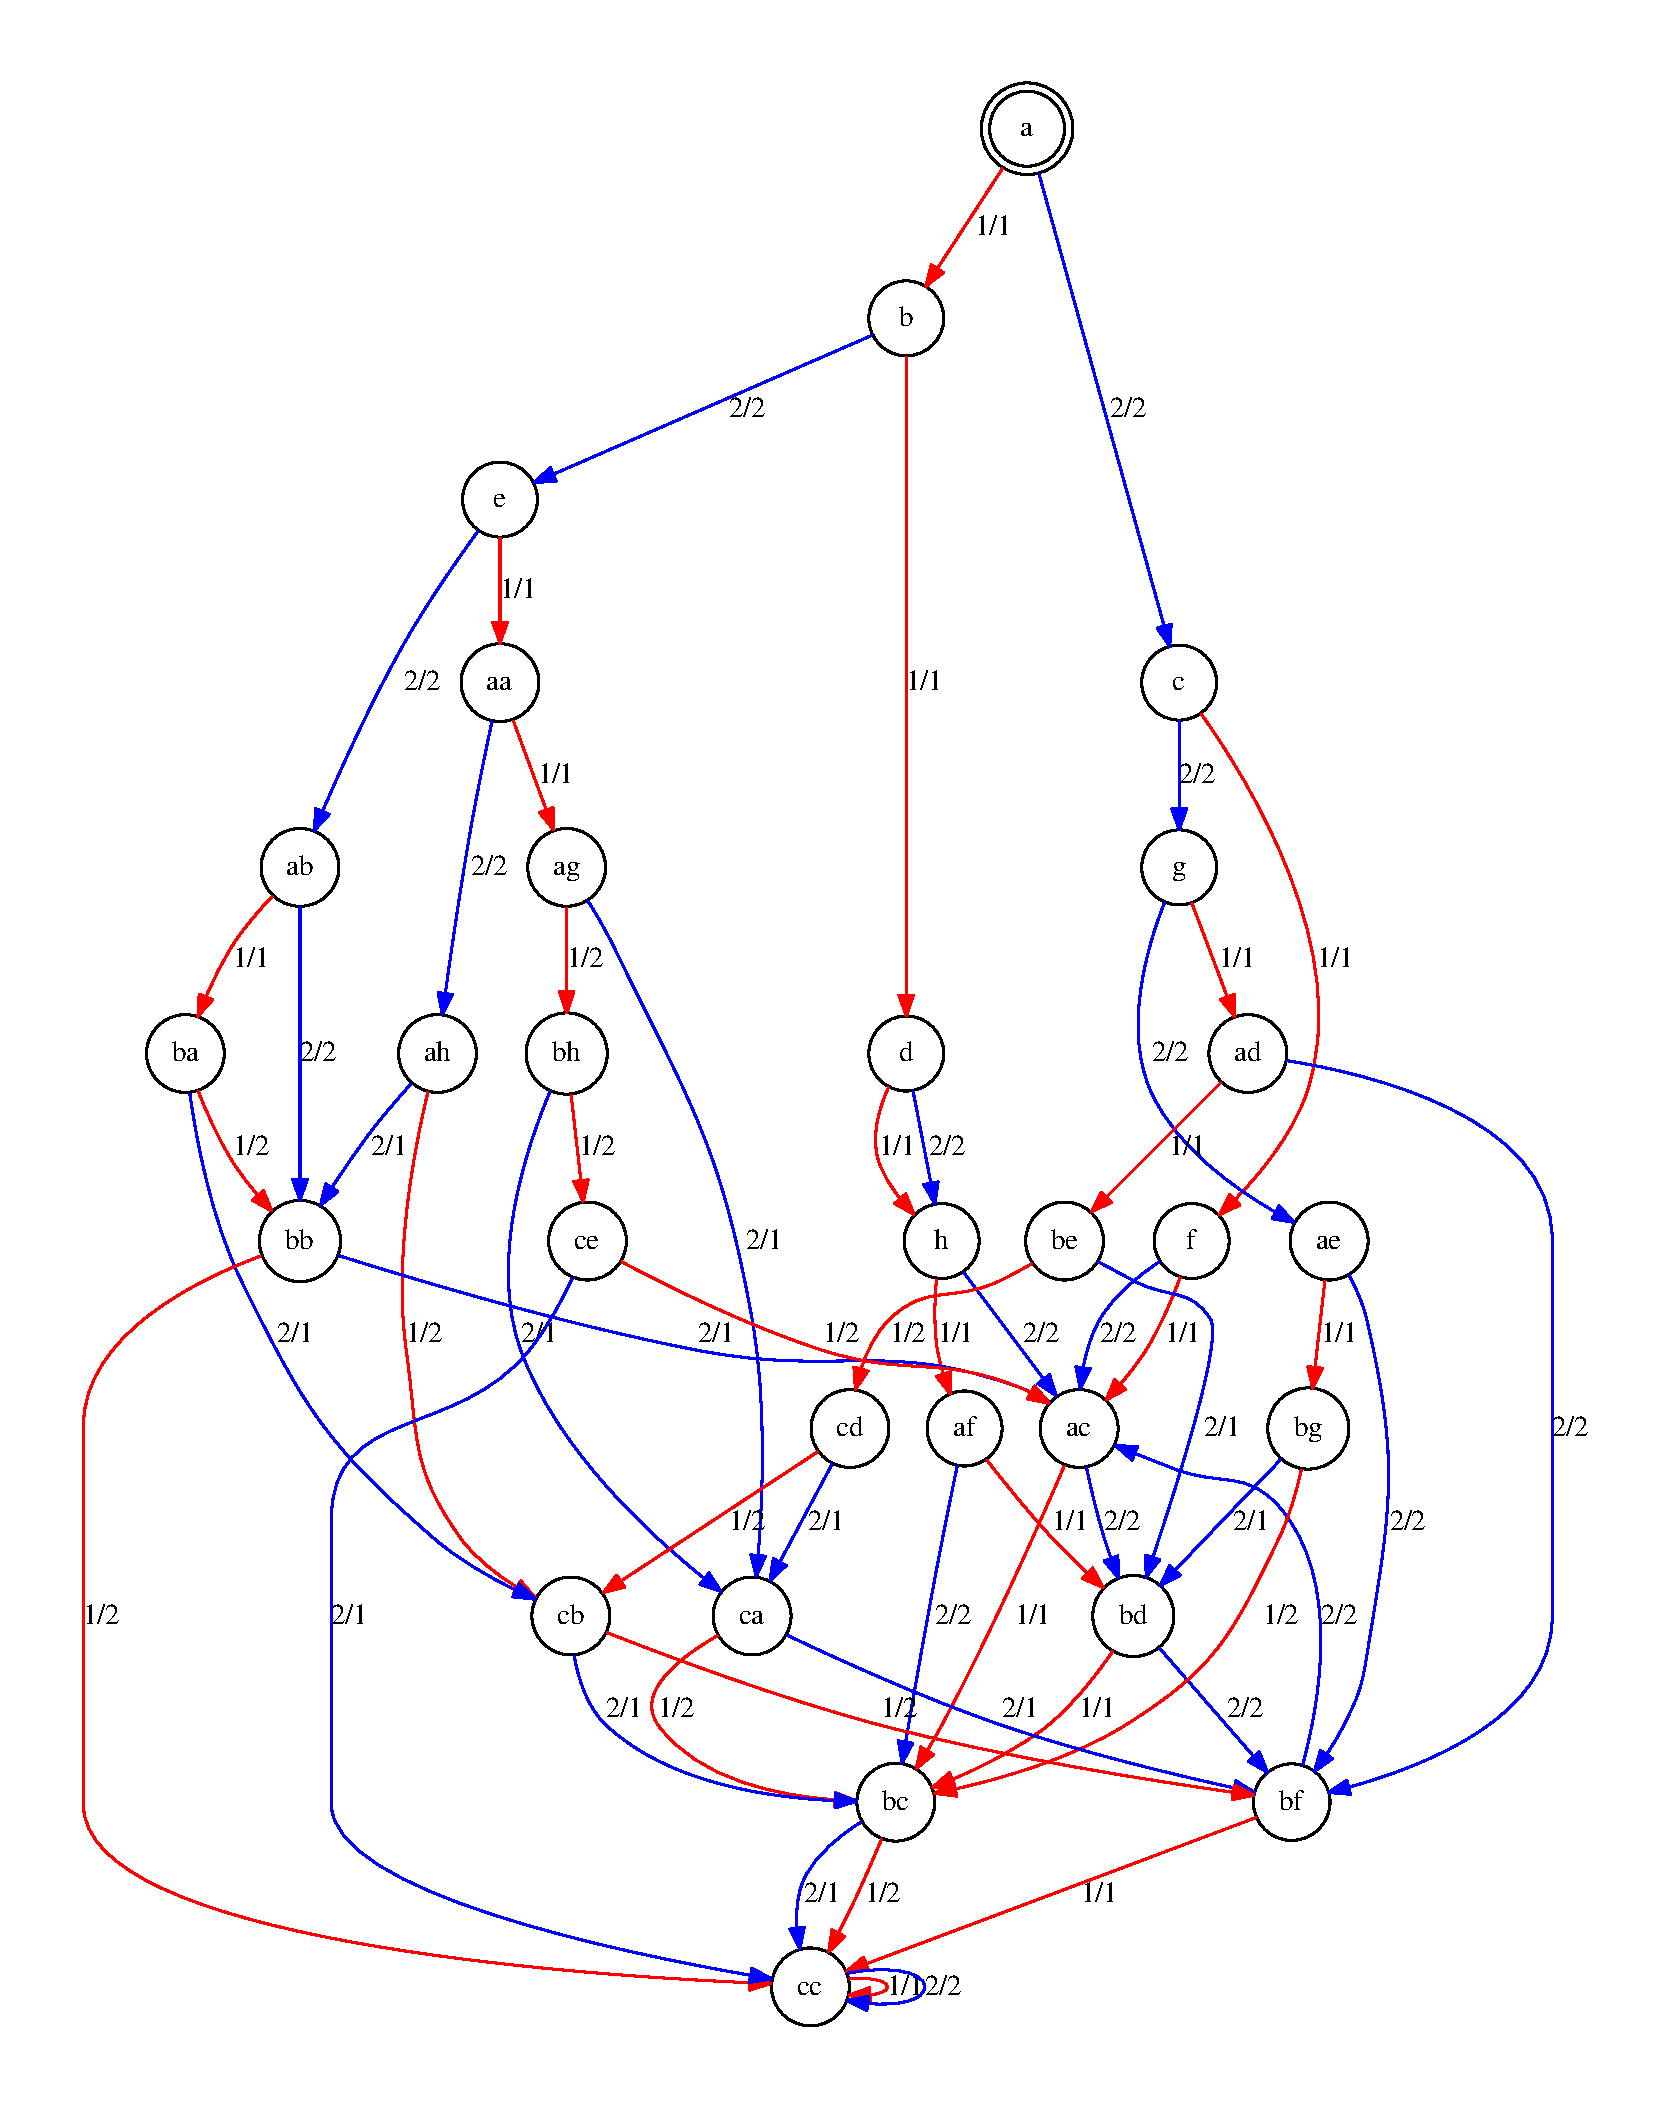
\includegraphics[width=\textwidth]{gap/PCD/noncomm29states}
 \caption{Element of the derived of the Grigorchuk group which is not a commutator.}\label{fig:noncomm}
\end{figure}
This finishes the proof of Theorem \ref{thm:CWGrigorchukGroup}.
\subsection{Bounded conjugacy width}
In \cite{Fink:Conjugacy_growth} it is proven that $G$ has finite bounded conjugacy width. Here we give an explicit bound 
on this width.
\begin{pro}
 Let $g$ be in $G'$. Then the equation 
 \begin{align*}
  a^{x_1}a^{x_2}a^{x_3}a^{x_4}a^{x_5}ag=1
 \end{align*}
is solvable in $G$. 
\end{pro}
\begin{proof}
We need to solve the equation $(E=a^{x_1}a^{x_2}a^{x_3}a^{x_4}a^{x_5}ag,\gamma)$ for
some constraint $\gamma$. Independent of the chosen constraint the replacement of
$x_i$ by $\pair{y_i,z_i}\act(\gamma(x_i)$ leads to an equivalent equation 
$R_2(g\at{2})(g\at{1})$. Similar to the construction of $\Gamma^q$ in the section
before one can find for each $q\in\RNK{G'}{K'}$ a constraint $\gamma$ such that
$\gamma(E^{\id*\pi})=1$ and $\gamma'\in\Gamma_1(\gamma)$ such that all for all 
$g\in\pi^{-1}(q)$ holds that $(g\at{2}g\at{1},\gamma')$ are good pairs.

Therefore the constrained equation $(R_2(g\at{2})(g\at{1}),\gamma')$ is solvable
for each $g\in G'$ and hence the equation $a^{x_1}a^{x_2}a^{x_3}a^{x_4}a^{x_5}ag$.

In GAP use the function \gapinline{verifyExistGoodConjugacyConstraints} to check this.
\begin{lem}
 There exits an element $g\in G'$ such that the equation 
 \begin{align*}
  a^{x_1}a^{x_2}a^{x_3}ag=1
 \end{align*}
 is not solvable.
\end{lem}
As before independent of the activities of a possible constraint $\gamma$ and of the element $g\in G'$
the normalform of $\Phi_\gamma(a^{x_1}a^{x_2}a^{x_3}ag)$ turns out to
be $R_1(g\at{2}) g\at{1}$. So all there is to prove is that there is an element $h\in K$
where the products of states $h\at{2}\cdot h\at{1}$ is not a commutator.

The element $g$ displayed in Figure \ref{fig:noncomm} provides such an element. It can easily be verified 
that $\pair{(cag)^\pi,(ac)^\pi}\in Q_1$ and $\omega(\pair{(cag)^\pi,(ac)^\pi})=1$. Thus by
the properties of the branch structure it is true that $\pair{(cag)^\pi,(ac)^\pi}\in K<G'$. 
\end{proof}
\begin{defi}[\cite{Fink:Conjugacy_growth}]
 The \emph{conjugacy width} of a group $G$ with generating set $S$ 
 is the least number $N\in\NN$ such that every element $g\in G$ is a product of
 at most $N$ conjugates of generators $s\in S$.
\end{defi}
\begin{cor}
 The Grigorchuk group $G$ with generating set $\{a,b,c,d\}$ has conjugacy width at most $8$.
\end{cor}
\begin{proof}
 The following set $T$ is a transversal of $\RNK{G}{G'}$. So every element $g\in G$ can be written as $g=th$ with $t\in T$ and $h\in G'$.
 \[T=\{1,a,d^aa,d^a,b,ab^a,ca^d,bd^a\}.\]
 As every element of $G'$ is a product of at most $6$ conjugates of $a$ this proofs the claim.
%  \begin{align}
%   T &=\{&1&,&a&,&ad=d^aa&,&ada=d^a,\\
%     & &b&,&ba=ab^a&,&bad=ca^d&,&bada=bd^a
%  \end{align}

\end{proof}

%TODO no need for this a.t.m.
% \begin{lem}
%  If $g\in K$ then 
%  \[(g\at{1},g\at{2})^{\pi\times\pi} \in \left\{\left(\left((ca)^n\right)^\pi,\left((ac)^n\right)^\pi\right) \mid n=1,\ldots,4\right\}\]
% \end{lem}







\section{Implementation in GAP}
\subsection{Usage of the attached files}
In the main directory of the archive you can type the command \gapinline{gap verify.g} and 
you will get as output a list of lemmata which are then proven to be true. 
The file calls all the previously mentioned methods \gapinline{verifi*}.
This approach uses
precomputed data which is also in the archive. This saves you a lot of computation time.

However you can recompute this data yourself if a sufficiently new version of GAP and
some packages are present. Inside the interactive gap shell after calling \gapinline{gap verify.g}
you can use the function \gapinline{RedoPrecomputation} with one argument. In each case
the result is written to a file and will override the original precomputed data. The 
argument can be one of the following:
\begin{itemize}
    \item [``orbits''] This will compute the $90$ orbits of $\RNK{\Aut(F_6)}{\Stab(R_3)}$ and the
		       $86$ orbits of $\RNK{\Aut(F_4)}{\Stab(R_2)}$. This computation will take
		       about $12$ hours on an ordinary machine and has no progress bar.
   \item [``goodpairs''] First this will compute for each constraint $\gamma\in\Red\cup\Red^4$ 
		      the set of all $q\in\RNK{G'}{K'}$ such that $(q,\gamma)$ is a good pair.
		      
		      Then it computes for each good pair $(q,\gamma)$ one $\gamma'\in\Gamma_q(\gamma)$
		      with decorated $x=y_{\gamma'}\in S$ as defined in \ref{def:Gammaq} which 
		      fulfills depending whether $\gamma\in\Red^4_{act}$ or $\gamma\in\Red_{act}$ 
		      either Proposition \ref{pro:existsNextPair} or Proposition \ref{pro:existsNextPair4}.
		      This computation will take about $2$ hours on ordinary machines and is equipped 
		      with a progress bar. 
		      
		      Afterwards the successor of $(q,\id)$ is computed which is needed for 
		      Corollary \ref{cor:KhasCW2}. 
   \item [``conjugacywidth''] Denote by $E_g$ the equation $a^{x_1}a^{x_2}a^{x_3}a^{x_4}a^{x_5}ag$.
		      For each $g^\tau=q\in\RNK{G'}{K'}$ this will compute a constraint 
		      $\gamma\colon F_5 \to Q$ for the equations $E_g$
		      and a constraint $\gamma'\colon F_4\to Q$ such that
		      $(\gamma * \pi)(E_g) = 1$ and 
		      \[E'_g := \nf(\Phi_\gamma(E_g))=[x_1,x_2][x_3,x_4](g\at{2})(g\at{1}).\] and
		      $(E'_g,\gamma')$ is a good pair for all $g$ with $g^\tau=q$.
		      
		      The computation will take about one hour and is equipped with a progress bar.
  \item [``all''] This will do all of the above one after another.		      
   \end{itemize}
If you are going to recompute the orbits GAP should be started with the \gapinline{-o} flag
to provide enough memory for the computation. For example start GAP by 
\gapinline{gap -o 8G verify.g}


\subsection{Implementation details}
\label{sec:gap_details}
\subsubsection{Reduced Constraints}
The proof of Lemma \ref{lem:finitelyManyConstraints} in \cite{Lysenok:QudraticEquationsInGrig} 
provides a constructive method to reduce any constraint to one with support
only in the first five variables. 
We have implemented this in the function \gapinline{ReducedConstraintAllModes} in the file
\filename{gap/functions.g}.

It uses that the quotient $Q=\RNK{G}{K}$ is a polycyclic group with 
\begin{align*}
 C_0 &= Q = \left<a^\pi,b^\pi,d^\pi\right>, &
 C_1 &= \left<a^\pi,d^\pi\right>, &
 C_2 &= \left<(ad)^\pi\right>.
\end{align*}
We take the generators of $\Stab(R_n)$ as given in the proof of Lemma \ref{lem:90Constraints}
plus additional ones which can switch two neighboring pairs:
\begin{align*}
 s_i &\colon &x_i&\mapsto x_{i+2}&\\
	    &&x_i+1&\mapsto x_{i+3}&\\
	    &&x_i+2&\mapsto x_{i}^{[x_{i+2},x_{i+3}]}&\\
	    &&x_i+3&\mapsto x_{i+1}^{[x_{i+2},x_{i+3}]} & \textup{ for }i = 1,3,\ldots,2n-3.
\end{align*}
It can easily be checked, that these are also contained in $\Stab(R_n)$. These elements
are used to reduce a given constraint in a form of a list with entries in $Q$ to a
list where all entries with index larger then $5$ are one. 
This constraint can then be further reduced by a lookup table for the orbits
of $\RNK{\Aut(F_6)}{\Stab(R_3)}$. 

If the file \filename{verify.g} is loaded in a GAP environment with the FR package available 
the function \gapinline{ReducedConstraint} can be used as an alias to get 
reduced constraints. For Example:
 \begin{lstlisting}
    f4 := Q.1; f2 := Q.2;
    gamma:= [f1,f1,f1,f1,f1,f1];
    constr := ReducedConstraint(gamma);;
    Print(constr.constraint);
\end{lstlisting} 
\begin{verbatim}
>>>      [ <id>, <id>, <id>, <id> , f4, <id>]
\end{verbatim} 

\subsubsection{Good pairs}
For $g\in G$ and a constraint $\gamma$ the question if $(g,\gamma)$ is a good
pair depends only on the image $g^\tau\in\RNK{G}{K'}$ and the representative
of $\gamma\in\Red$. (See Section \ref{sec:good_pairs}.) So this is already a
finite problem. 

For a given constraint $\gamma$ to get all $q$ which form a good pair we can
enumerate all possible commutators for $r_i\in\varpi^{-1}(\gamma(x_i)$.
$[r_1,r_2][r_3,r_4][r_5,r_6]$. Since $\lvert\RNK{K}{K'}\rvert=64$ considering all 
combinations at once is far from beeing efficient thus the possible values for
$[r_1,r_2]$ are computed and in a second step products of those elements.
This is implemented in the function \gapinline{goodPairs} in the file
\filename{gap/functions.g}.
\subsubsection{Successors}
The key ingredient for the proof of Theorem \ref{thm:CWGrigorchukGroup} is
Proposition \ref{pro:existsNextPair}. The computational effort there is
to compute the sets $\Gamma_q(\gamma)$ and find good pairs inside of them.

This is implemented exactly as explained in the construction of the map
$\Gamma_q$ in the function \gapinline{GetSuccessor} in the file 
\filename{gap/precomputeGoodPairs.g}. Given an element $q\in\RNK{G'}{K'}$ 
and an active constraint $\gamma$ this function returns a tuple $(\gamma',x)$ 
with $\gamma\in\Red$ and $x$ the decorated element $y_\gamma'$.

Given an inactive constraint $\gamma$ it returns a pair of constraints
$\gamma_1,\gamma_2$ such that both have nontrivial activity and with
$\omega$ the map from the branch structure it hold:
$\omega(\pair{\gamma_1(x_i),\gamma_2(x_i)})=\gamma(x_i)$. 

If the FR package is available
the function \gapinline{GetSuccessorLookup} can be used to explore the
successors of elements. It returns the successing pair. For example
 \begin{lstlisting}
    f1 := Q.1; f2 := Q.2;
    gamma:= [f1,f1,f1,f1,f1,f1];;
    g := (a*b)^8;;
    IsGoodPair(g,gamma);
\end{lstlisting}
\begin{verbatim}
>>>      true
\end{verbatim} 
\begin{lstlisting}
    suc := GetSuccessorLookup(g,gamma);;    
    suc[1];
\end{lstlisting}
\begin{verbatim}
>>>      <Trivial Mealy element on alphabet [ 1 .. 2 ]>
\end{verbatim} 
\begin{lstlisting}
    suc[2].constraint;
\end{lstlisting}
\begin{verbatim}
>>>       [ <id>, <id>, <id>, <id>, f1*f2, <id> ]
\end{verbatim} 



%\paragraph{Lemma \ref{lem:atIsWellDefinedModK'}}
%\paragraph{Lemma \ref{lem:existsGoodGamma}}

\bibliography{latex/bio}
\appendix
% \include{Abschnitte/Anhang}
%\include{Abschnitte/Erklaerung}


\end{document}
